 %%%%%%%%%%%%%%%%%%%%%%%%%%%%%%%%%%%%%%%%%%%%%%%%%%%
%\documentclass[graybox, envcountchap]{Structure/Preamble/svmult}
%\usepackage{amssymb}
\usepackage{amsmath}

\usepackage[squaren]{SIunits}
\usepackage{breqn} %you need to load "breqn" after "SIunits", else i got problems on a decimal point in equations which disappear.

\usepackage{color} % defines colors to be used for highlighting
\usepackage{dtsyntax} % recognizes modelica code
%\usepackage{cite} % to order references properly
\usepackage[table]{xcolor}

%for postprocessing matplotlib figures with the appropriate font
\usepackage{pgf}
\usepackage{pgfplots}

%COLORS
\definecolor{KulBlue}{RGB}{16,67,122}

%net
\textheight 19.3cm %19.3cm	% vele andere: slechts 17.5 
\textwidth 13cm %12.3cm  	%lode zelfs 12.5
\oddsidemargin 1.5cm
\evensidemargin 1.5cm

%figures 
\usepackage{graphicx}

% listings
\usepackage{listings}
\renewcommand\lstlistlistingname{List of Listings} % default is Listings
\lstset{language=JAVA}

% programming code listings
\usepackage{listings}

% boxedverbatim
\usepackage{moreverb}

\usepackage[xetex, bookmarks, colorlinks, breaklinks, pdftitle={Ruben Baetens - vita},pdfauthor={My name}]{hyperref}  
\hypersetup{linkcolor=KulBlue,citecolor=KulBlue,filecolor=black,urlcolor=KulBlue} 

\usepackage{mathptmx}
\usepackage{helvet}
\usepackage{courier}
%
\usepackage{type1cm}         

\usepackage{makeidx}         % allows index generation
\usepackage{graphicx}        % standard LaTeX graphics tool
                             % when including figure files
\usepackage{multicol}        % used for the two-column index
\usepackage[bottom]{footmisc}% places footnotes at page bottom

% see the list of further useful packages
% in the Reference Guide

\makeindex             % used for the subject index
                       % please use the style svind.ist with
                       % your makeindex program

\usepackage{subfigure}

\newcounter{tmpc}



\documentclass[final]{phd}
\bibliographystyle{ieeetr}

\usepackage{pdfsync} 
\hypersetup{pdfstartpage=1,% TODO: nakijken en aanpassen in definitieve versie
	pdftitle={Building optimisation for energy system integration},%
	pdfauthor={Ruben Baetens},%
	pdfsubject={UDC 519.65, 681.3*G16, 681.3*I6}}

%%%%%%%%%%%%%%%%%%%%%%%%%%%%%%%%%%%%%%%%%%%%%%%%%%%%%%%%%%%%%%%%%%%%%

\newcommand{\Qflow}{\boldsymbol{Q}}
\newcommand{\qflow}{\boldsymbol{q}}
\newcommand{\T}{\boldsymbol{T}}
\newcommand{\s}{(k)}

\newcommand{\eg}{\mbox{\emph{e.g.\ }}}
\newcommand{\etal}{\mbox{\emph{et al.\ }}}
\newcommand{\ie}{\mbox{\emph{i.e.\ }}}
\newcommand{\fixme}{\textcolor{red}{\textbf{fixme}}\ }

\newcommand{\abb}[1]{\textsc{#1}}
\newcommand{\name}[1]{#1}
\newcommand{\yr}[1]{\oldstylenums{#1}}
\newcommand{\quo}[1]{\emph{#1}}

\newcommand{\tv}[1]{\boldsymbol{#1}}
\newcommand{\tim}{}

\begin{document}

\maxtocdepth{chapter}
\maxsecnumdepth{subsubsection}
\pagestyle{empty}
\pagenumbering{alph}


%%   FRONT PAGE       %%
%%%%%%%%%%%%%%%%%%%%%%%%
% 
 \thispagestyle{empty}   % no headings for this page
% 
% % Header
 \noindent
 \begin{minipage}{3cm}%
   \includegraphics*[width=2.5cm]{figures/KULeuvenlogo.pdf}% logo ku leuven
 \end{minipage}\hfill
 \begin{minipage}{8cm}
 \raggedleft
 \small{KU Leuven\\
 Faculteit Ingenieurswetenschappen}
 \end{minipage}
% 
% % Title
\\[2cm]
   \begin{flushleft}
     \large \textbf{IDEAS.mo}\\
     \vspace{0.1in}\large{Integrated District Energy Assessment Simulations}%\noindent
   \end{flushleft}
 \hrule
% 
 \bigskip
   \large\noindent \small{Ruben Baetens, Roel De Coninck, Bart Verbruggen, Juan Van Roy, \\ Johan Driesen, Lieve Helsen, Dirk Saelens} \hfill
 \bigskip
% 
% % Footer
 \vfill
 \begin{minipage}{2.0cm}%
     \includegraphics*[width=2.0cm]{figures/sedes.pdf}% 
 \end{minipage}\hfill
 \begin{minipage}{9cm}
 \raggedleft
% \small{Dissertation presented in partial\\
% fulfillment of the requirements for\\
% the degree of Doctor in Engineering Science\\
% dd xx.xx.2014
% }
 \end{minipage}

\clearpage{\pagestyle{empty}\cleardoublepage}


\frontmatter%%%%%%%%%%%%%%%%%%%%%%%%%%%%%%%%%%%%%%%%%%%%%%%%%%%%%%

\cleardoublepage
\pagestyle{fancy}

\chapter*{Contents}
\renewcommand\contentsname{}
\makeatletter
\@starttoc{toc}
\makeatother

%\tableofcontents
%%%%%%%%%%%%%%%%%%%%%clist.tex %%%%%%%%%%%%%%%%%%%%%%%%
%                                                    
% sample list of contributors and their addresses    
%                                                    
% Use this file as a template for your own input.    
%                                                    
%%%%%%%%%%%%%%%%%%%%%%%% Springer %%%%%%%%%%%%%%%%%%%%
\contributors

\begin{thecontriblist}
Ruben Baetens \at K.U.Leuven, Kasteelpark Arenberg 40 bus 2447, BE-3001 Leuven (Heverlee) \email{ruben.baetens@bwk.kuleuven.be}
\and
Roel De Coninck \at K.U.Leuven, Celestijnenlaan 300a bus 2421, BE-3001 Leuven (Heverlee) \email{roel.deconinck@mech.kuleuven.be} 
\and
Juan Van Roy \at K.U.Leuven, Kasteelpark Arenberg 10 bus 2445, BE-3001 Leuven (Heverlee) \email{juan.vanroy@esat.kuleuven.be} 
\and
Bart Verbruggen \at K.U.Leuven, Kasteelpark Arenberg 10 bus 2445, BE-3001 Leuven (Heverlee) \email{bart.verbruggen@esat.kuleuven.be} 
\and
Johan Driesen \at K.U.Leuven, Kasteelpark Arenberg 10 bus 2445, BE-3001 Leuven (Heverlee) \email{johan.driesen@esat.kuleuven.be} 
\and
Lieve Helsen \at K.U.Leuven, Celestijnenlaan 300a bus 2421, BE-3001 Leuven (Heverlee) \email{lieve.helsen@mech.kuleuven.be} 
\and
Dirk Saelens \at K.U.Leuven, Kasteelpark Arenberg 40 bus 2447, BE-3001 Leuven (Heverlee) \email{dirk.saelens@bwk.kuleuven.be}
\end{thecontriblist}


\mainmatter

%\begin{partbacktext}
\part{Specifications}
%\noindent spec-i-fi-ca-tion (n.) 1. the act of specifying. 2. a. specifications, A detailed, exact statement of particulars, especially a statement prescribing materials, dimensions, and quality of work for something to be built, installed, or manufactured. b. A single item or article that has been specified. 3. An exact written description of an invention by an applicant for a patent.
%\end{partbacktext}


\chapter{Climate}
%\title{Climate}


%\author{Ruben Baetens and Dirk Saelens}
%\authorrunning{R. Baetens, D. Saelens}
%\institute{Ruben Baetens \at KU Leuven, Kasteelpark Arenberg 40 bus 2447, BE-3001 Leuven (Heverlee) \email{ruben.baetens@bwk.kuleuven.be}
%\and Dirk Saelens \at KU Leuven, Kasteelpark Arenberg 40 bus 2447, BE-3001 Leuven (Heverlee) \email{dirk.saelens@bwk.kuleuven.be}}
%\maketitle

%\abstract{A numeric building model is developed in Modelica for integrated energy simulation.}

%\vspace{\baselineskip}

In this section, we describe in detail the climate model and its possibilities that are implemented in Modelica as part of the IDEAS platform. Four external factors are to be known, i.e. external temperature and ground temperature for transient heat losses by conduction, sky temperature for long-wave radiation losses and short-wave gains on surfaces by solar irradiation.


\section{Climate conditions}

In this section, we describe in detail the climate model and its possibilities that are implemented in Modelica as part of the IDEAS platform. Four external factors are to be known, i.e. external temperature and ground temperature for transient heat losses by conduction, sky temperature for long-wave radiation losses and short-wave gains on surfaces by solar irradiation.

\subsection{Weather data}
\label{chap:climwea}

The main weather parameters required for transient thermal building simulation are the ambient dry-bulb temperature $T_{db}(t)$, the outdoor relative humidity $\varphi_{e}(t)$, the wind speed $v_{10}(t)$, the diffuse horizontal solar radiation $E_{d,h}(t)$ and direct normal solar radiation$E_{D,\bot}(t)$. 

The Meteonorm system~\cite{Meteotest2008} is a comprehensive source of (all mentioned) weather data for engineering applications in Europe and this system is used within this context. For simulation, the retrieved data from the Meteonorm system are not used within the common formats of a test reference year \texttt{*.try}~\cite{NCDC1981,EC1985} as used in Europe or the formats of a typical meteorological years \texttt{*.tmy} or \texttt{*.tmy2}~\cite{NCDC1976b,NREC1995} and weather years for energy calculations \texttt{*.wyec} or \texttt{*.wyec2}~\cite{ASHRAE1985} as used in the United States and Canada. These data formats are derived from hourly observations at a specific location by the national weather service or meteorological office and contain too little information for sub-hourly simulation, especially towards renewable energy generation by solar radiation.

From the retrieved data from the Meteonorm system, one more temperature needs to be determined. The long-wave radiative heat exchange of an exterior surface with a cloudy sky is calculated based on a sky temperature. This black-body sky temperature $\T_{ce}$ can be determined~\cite{Walton1983,Martin1984} as \\*
\begin{gather}
\T_{ce}=\T_{db} \sqrt[4]{\boldsymbol{\varepsilon}_{ce}} \\
\boldsymbol{\varepsilon}_{ce} = \boldsymbol{\varepsilon}_{ce,0}+\boldsymbol{C}_{cf} \boldsymbol{\varsigma}_{ce,0}
\end{gather}
where $\boldsymbol{\varepsilon}_{ce}$ is the cloudy sky emissivity~\cite{Berdahl1982,Berdahl1984,Martin1984}, where $\boldsymbol{\varepsilon}_{ce,0}$ is the clear sky emisivity and $\boldsymbol{C}_{cf}$ is the cloud cover factor. Both  $\boldsymbol{\varepsilon}_{ce,0}$ and $\boldsymbol{C}_{cf}$ are determined as polynomial fits on measurement data: \\*
\begin{gather}
\boldsymbol{\varepsilon}_{ce,0} \varpropto 0.711 + 0.0056\ \boldsymbol{\vartheta}_{dw} + 0.000073\ \boldsymbol{\vartheta}_{dw}^{2} + 0.013\ \cos \boldsymbol{h} \\
\boldsymbol{C}_{cf} \varpropto 1.0 + 0.024\ \boldsymbol{C}_{c} - 0.0035\ \boldsymbol{C}_{c}^{2} + 0.00028\ \boldsymbol{C}_{c}^{3}
\end{gather}
where $\boldsymbol{h}$ is the hour angle, $\boldsymbol{\vartheta}_{dw}$ is the dew temperature and $\boldsymbol{C}_{c}$ is the tenths cloud cover retrieved from Meteonorm~\cite{Kasten1979,Perraudeau1990}. 

\subsection{Solar radiation}
\label{chap:climsol}

The calculation of the direct and diffuse solar irradiation on a tilted surface requires determination of the position of the sun in the sky. Here, the zenith angle $\xi(t,x)$ of surface with inclination $i(x)$ and azimuth $a(x)$ are able to uniquely define the the solar radiation on a tilted surface based on the determination of the annual and daily solar cycle by means of solar time and declination.

Within the computational model, all solar irradiation calculations are handled in \texttt{Commons.Meteo.Solar.RadSol} which is built-in in each surface receiving solar radiation.

\subsubsection{Solar geometry}

The apparant solar time $\boldsymbol{t}_{sol}$ expressed in seconds is based on daily apparent motion of the sun as seen from the earth. Solar noon is defined as the moment when the sun reaches the highest point in the sky. Solar time defined as \\*
\begin{gather}
\boldsymbol{t}_{sol} = \boldsymbol{t}_{std} + 720\pi^{-1}\left(L_{std}-L_{loc}\right) + \boldsymbol{E}_{t} \\
\boldsymbol{E}_{t} = -120\ e\sin \boldsymbol{M} + 60\tan^{2} \left(\varepsilon/2\right) \sin \left(2\boldsymbol{M}+2\lambda_{p}\right)
\end{gather}
where $\boldsymbol{t}_{std}$ is the standard time of the time zone, $L_{std}$ is the reference meridian, $L_{loc}$ is the lcoal meridian and $\boldsymbol{E}_{t}$ is the equation of time defining the difference between solar noon and noon of local civil time, $\boldsymbol{M}$ is the mean anomaly relating to the position of the sun to the earth in a Kepler orbit, $\varepsilon$ is the earth obliquity and $\lambda_{p}$ the ecliptic longitude of the periapsis, \ie, the closest approach of the earth to the sun. Daylight saving time is taken into account within the simulation and corrects $\boldsymbol{t}_{std}$. Daylight saving time starts in the European Economic Community on March $31-\left[(5y)/4+4\right]$ mod $7$ and ends on October $31-\left[(5y)/4+1\right]$ mod $7$ where $y$ denotes the year and mod denotes the remainder by division~\cite{VanGent2011}.

Before the zenith angle can be calculated, the declination $\boldsymbol{\delta}$ and solar hour angle $\boldsymbol{h}$ is to be defined to fully specify the position of the sun as seen by an observer at a given time. Here, $\boldsymbol{\delta}$ depicts the angle between the solar beam and the equatorial plane, defined~\cite{Spencer1971} as \\*
\begin{equation}
\sin \boldsymbol{\delta} = \sin \varepsilon \cos \left(2\pi \left(\boldsymbol{n}+10\right) n_{y}^{-1} \right)
\end{equation}
where $\varepsilon$ is the earth obliquity, $n(t)$ is the one-based day number, i.e. 1 for January 1, and $n_{y}$ is the length in days of the earth revolution equal to 365.25 days. The correction of 10 days is required as winter solstice, i.e. when the apparent position of the sun in the sky as viewed from the Earth reaches its most northern extreme, occurs at December 21. 

The hour angle $\boldsymbol{h}$ depicts the angle between between the half plane of the Earth's axis and the zenith and the half plane of the Earth's axis and the given location, defined as  \\*
\begin{equation}
\boldsymbol{h} = 2\pi \boldsymbol{t}_{sol}\ 86400^{-1} - \pi
\end{equation}
where $\boldsymbol{t}_{sol}$ is solar time.

Based on $\boldsymbol{\delta}$ and $\boldsymbol{h}$, the zenith angle $\boldsymbol{\xi}^{\s}$ of a surface $k$ can be uniquely defined. The zenith angle of the sun to a surface is the angle between this surface normal and the sun's beam, and is derived from~\cite{Duffie1980,Iqbal1983} \\*
\begin{equation} 
\cos\boldsymbol{\xi}^{\s}=\sin\boldsymbol{\delta}  \sin\varphi  \cos i^{\s}-\sin\boldsymbol{\delta}  \cos\varphi  \sin i^{\s} \cos a^{\s}+\cos\boldsymbol{\delta} \cos\varphi  \cos i^{\s} \cos a^{\s} + \\ \cos\boldsymbol{\delta}  \cos \boldsymbol{h}  \sin\varphi  \sin i^{\s}  \cos a^{\s} +\cos\boldsymbol{\delta}  \sin \boldsymbol{h} \sin i^{\s} \sin a^{\s} 
\end{equation}
where $\varphi$ is the latitude of the location defined positive for the northern hemisphere, $\boldsymbol{h}$ is the hour angle, $i^{\s}$ is the surface inclination defined as 0 for ceilings and $\pi/2$ for vertical walls, $a^{\s}$ is the surface azimuth defined as $-\pi/2$ if the surface outward normal points eastward and 0 if the normal points southward, and where $\boldsymbol{\delta}$ is the solar declination.

\subsubsection{Shortwave radiation on a tilted surface}

The total solar irradiation $E(t,x)$ on a arbitrary surface can be determined as the sum of the direct $E_{D}(t,x)$, diffuse $E_{d}(t,x)$ and reflected $E_{r}(t,x)$ radiation on the surface.  \\*
\begin{equation}
E(t,x)=E_{D}(t,x)+E_{d}(t,x)+E_{r}(t,x)
\end{equation}
For a known profile of direct solar irradiation on a random surface, all three factors can be determined for another arbitrary surface s. Herefore, a profile of direct solar irradiation $E_{D,\bot}(t,x)$ perpendicular on the beam radiation is retrieved from Meteonorm and used as only input parameter. The calculation of other configurations besides normal to the solar beam is performed in the model. 

Different models for the determination of the diffuse radiation do exist based on an isotropic or anisotropic model of the sky dome. On account of the high importance of solar irradiation for the model\footnote{Solar radiation interacts e.g. with the building thermal response, heat generation by means of a thermal solar collector and power generation with a photovoltaic array}, a more detailed determination of diffuse radiation based on a anisotropic sky dome model is favorable. Herefore, the Perez model~\cite{Perez1986,Perez1987} is implemented.  \\*
\begin{gather}
E_{d}(t,x) =  A(x) E_{d,h}(t) \left[ 0.5 \left(1+\cos i\right) \left(1-F_{1}\right) + F_{1} \cos\xi(t,x) \cos^{-1}\xi_{h}(t) + F_{2} \sin i\right]  \\
E_{r}(t,x) = 0.5 \rho A(x) \left(E_{D,h}(t) + E_{d,h}(t)\right) \left(1 - \cos i\right)
\end{gather}

wherefore $A(x)$ is the surface area, $E_{d,h}$ is the diffuse horizonal radiation, $i$ is the surface inclination, $F_{1}$ is the circomsolar brightening coefficient, $F_{2}$, $\rho$ is the ground reflectance and $E_{D,h}$ is the direct horizonal radiation. The brightening coefficients $F_{1}$, $F_{2}$ are determined as \\*
\begin{equation}
F_{n} = F_{n,1}(\varepsilon) + F_{n,2}(\varepsilon) \Delta + F_{n,3}(\varepsilon) \xi_{h}(t)
\end{equation}
where $F_{n,i}$ are determined in the Perez model~\cite{Perez1987} based on measurements, $\varepsilon$ is the sky clearness and $\Delta$ is the sky brightness. Here, the sky brightness $\Delta$ is determined as $E_{d,h} E_{sc}^{-1}$ while the sky clearness $\varepsilon$ is determined as \\*
\begin{equation}
\varepsilon = \left(E_{d,h}(t,x) + E_{D,h}(t,x)\right) E_{d,h}(t,x)^{-1} + \kappa \xi_{h}^{3}(t) \left(1 + \kappa \xi_{h}^{3}(t)\right)^{-1}
\end{equation}
wherefore $E_{sc}$ is the solar constant and $\kappa$ equals 1.041.

\subsubsection{Solar shading}

So far, two types of structures which can shade a surface and thus reduce the shortwave radiation on a surface, i.e. an exterior screen in the pane of the surface and surface overhangs.

%\runinhead{Exterior solar screen.} 
The implementation of an exterior solar screen in the surface pane is stratightforward. The transmitted direct solar irradiation equals $E_{D}(t,x) \left(1 - f_{p}(t)\right)$ where $f_{p}(t)$ is the position of the screen between 0 and 1. The total transmitted diffuse and reflected solar irradiation equals $E_{d}(x,t) \left(1 - f_{p}\right) +f_{p}(t)  f_{s} E(x,t)$ where $f_{sha}$ is the shortwave transmittance of the exterior screen.

%\runinhead{Overhangs for vertical surfaces.} 
Horizontal and vertical projectionso above and besides windows are able to intercept the direct component of solar radiation depeneding on the geometry of the obstructing and receiving surface. The usnlit area $A_{SL}(x,t)$ of a surface with width $W$ and height $H$, and vertical and horizontal projections $P_{V}$ and $P_{H}$ at a distance $R_{W}$ and $R_{H}$ of the receiving surface edges is determined as  \\*
\begin{equation}
A_{SL}(x,t) = \left[W - P_{v}  \left|\tan \alpha(t,x) \right| + R_{W}\right] \left[H - P_{H} \tan \left(\pi - \xi_{h}(t)\right) \cos^{-1} \alpha(t,x) + R_{H}\right]
\end{equation}
with $\alpha(t,x)$ the solar azimuth.














\chapter{Transient building response model}
% Use \titlerunning{Short Title} for an abbreviated version of your contribution title if the original one is too long
%\author{Ruben Baetens and Dirk Saelens}
%\authorrunning{R. Baetens, D. Saelens}
%\institute{Ruben Baetens \at K.U.Leuven, Kasteelpark Arenberg 40 bus 2447, BE-3001 Leuven (Heverlee) \email{ruben.baetens@bwk.kuleuven.be}
%\and Dirk Saelens \at K.U.Leuven, Kasteelpark Arenberg 40 bus 2447, BE-3001 Leuven (Heverlee) \email{dirk.saelens@bwk.kuleuven.be}}
%\maketitle

%\abstract{A numeric building model is developed in Modelica for integrated energy simulation.}

%\vspace{\baselineskip}

\section{Introduction}

\section{Building thermal response}

% From an engineering point of view, the building is an energy sink in response to the outdoor climate and to be kept at potentials set by its occupants and health standards.

In this section, we describe in detail the dynamic building model and its possibilities that are implemented in Modelica as part of the \textsc{ideas} platform. The building model allows simulation of the energy demand for heating and cooling of a multi-zone building, energy flows in the building envelope and interconnection with dynamic models of thermal and electrical building energy systems within the platform for comfort measures. 

The description is divided into the description of the \index{wall} model and the \index{zone} model. The window model and the model for ground losses are described more in detail as extend to the wall model.

The relevant material properties of the surfaces are complex functions of the surface temperature, angle and wavelength for each participating surface. The assumptions used frequently in engineering applications~\cite{Walton1983} are that [``each surface emits or reflects diffusely and is at a uniform temperature''] and [``the energy flux leaving a surface is evenly distributed across the surface and one-dimensional'']. 

\subsection{Parallel opaque layers}

The description of the thermal response of a \index{wall} or a structure of parallel opaque layers in general is structured similar to the different occurring processes, \ie, the heat balance of the exterior surface, the heat balance of the interior surface and the heat conduction between both surfaces.

\subsubsection{Exterior surface heat balance}

The heat balance of the exterior surface $k$ is determined as \\*
\begin{equation}
\qflow_{cd}^{\s} + \qflow_{cv}^{\s} + \qflow_{sw}^{\s} + \qflow_{lw,e}^{\s} = 0
\end{equation}
where $\qflow_{cd}^{\s}$ denotes the conductive heat flow into the wall, $\qflow_{cv}^{\s}$ heat transfer by convection, $\qflow_{sw}^{\s}$ shortwave absorption of direct and diffuse solar light, $\qflow_{lw,e}^{\s}$ longwave heat exchange with the environment including the sky.

\paragraph{Convection}
We define the exterior convective heat flow between the exterior surfaces and the outdoor air based on an convective heat transfer coefficient as \\*
\begin{gather}
\qflow_{cv}^{\s} = \boldsymbol{h}_{cv}^{\s} \left(\T_{db,e} - \T_{s}^{\s}\right) \label{eq:qcve} \\
\boldsymbol{h}_{cv}^{\s} = \widetilde{\max}\left\{5.01\ \boldsymbol{v}_{10}^{0.85},\,5.6 \, ; \, 0.1\right\} \ \textrm{W}/\textrm{m}^{2}\textrm{K} \label{eq:hce}
\end{gather}
where $\T_{db,e}$ is the outdoor dry-bulb air temperature, $\T_{s}^{\s}$ is the surface temperature and $\boldsymbol{h}_{cv}^{\s}$ is the exterior convective heat transfer coefficient as defined in eqn. \ref{eq:hce} where $\boldsymbol{v}_{10}$ (\metre\per\second) is the wind velocity in the undisturbed flow field at 10 meter above the ground. The stated correlation with $\boldsymbol{v}_{10}$ is introduced to account for buoyancy driven convection at low wind velocities and forced convection induced by increasing velocities, and is valid for a $\boldsymbol{v}_{10}$ range of \mbox{$\left[0.15,7.5\right]$ \metre\per\second}.\citep{Defraeye2011,Jurges1924}

\paragraph{Longwave radiation}
We define the longwave radiative heat flow between the exterior surface and the environment as \\*
\begin{equation}
\qflow_{lw,e}^{\s}=\sigma \varepsilon_{lw}^{\s} \left(\T_{s}^{\s,4} - F_{ce}^{\s} \T_{ce}^{4} - (1-F_{ce}^{\s}) \T_{db}^{4}\right)
\label{eq:qlwe}
\end{equation}
%\begin{equation}
%F_{ce}^{\s} = 
%\end{equation}
as derived from the Stefan-Boltzmann law wherefore $\sigma$ is the Stefan-Boltzmann constant, $\varepsilon_{lw}^{\s}$ is the longwave emissivity of the exterior surface, $F_{ce}^{\s}$ the radiant-interchange configuration factor between the surface and the celestial dome as defined in eqn. \ref{eq:Fce}, $\T_{s}^{\s}$ is the surface temperature and $\T_{db}$ and $\T_{ce}$ are the outdoor dry bulb and celestial dome temperature respectively.\citep{Stefan1879,Boltzmann1884,Mohr2008,Hamilton1952} The stated eqn. \ref{eq:qlwe} is derived under the assumption that the ground temperature equals the outdoor air temperature, and that we can treat the surrounding outer environment as a much larger enclosure compared to the surface area.

\paragraph{Shortwave radiation}
We define the absorbed shortwave solar irradiation by the exterior surface in relation to the incident irradiation as \\*
\begin{equation}
\qflow_{sw}^{\s}=\varepsilon_{sw}^{\s} \left( \boldsymbol{E}_{Sd}^{\s} + \boldsymbol{E}_{SD}^{\s} \right)
\end{equation}
where $\varepsilon_{sw}^{\s}$ is the shortwave absorption of the surface, and $\boldsymbol{E}_{Sd}^{\s}$ and $\boldsymbol{E}_{SD}^{\s}$ are respectively the diffuse and direct solar irradiation striking the depicted exterior surface as defined in eqns. \ref{eq:ESd,eq:ESD}. 

\subsubsection{Interior surface heat balance}
\label{sec:int}

The heat balance of the interior surface is determined as \\*
\begin{equation} \label{eq:intersurf}
\qflow_{cd}^{\s} + \qflow_{cv}^{\s} + \sum_{j \in \mathcal{J}^{\s}} \qflow_{sw,j}^{\s} + \sum_{j \in \mathcal{J}^{\s}} \qflow_{lw,j}^{\s} = 0
\end{equation}
where $\qflow_{cd}^{\s}$ denotes the heat flow into the wall, $\qflow_{cv}^{\s}$ te heat transfer by convection, $\qflow_{sw}^{\s}$ the shortwave absorption of direct and diffuse solar light entering the interior zone through windows and $\qflow_{lw}^{\s}$ the longwave heat exchange with the surrounding interior surfaces.

\paragraph{Convection}
We define the interior convective heat flow between the interior surfaces and zone air based on an convective heat transfer coefficient as \\*
\begin{gather}
\qflow_{cv}^{\s} = \boldsymbol{h}_{cv}^{\s} \left(\T_{db,i} - \T_{s}^{\s}\right) \\
\boldsymbol{h}_{cv}^{\s} = \widetilde{\max}\left\{1,\,n_{1}^{\s} D^{\s n_{2}^{\s}} \left|\T_{db,i}-\T_{s}^{\s}\right|^{n_{3}^{\s}} ;\, 0.1 \right\}
\label{eq:hcvi}
\end{gather}
similar to eqn. \ref{eq:qcve} with $\T_{db,i}$ the indoor dry-bulb temperature, $\T_{s}^{\s}$ the surface temperature and $\boldsymbol{h}_{cv}^{\s}$ the interior natural convective heat transfer coefficient. As the room-side heat transfer coefficient couples the room air temperature to the temperature of building components, detailed computation of its value is important. Therefore we define $\boldsymbol{h}_{cv}^{\s}$ as in eqn. \ref{eq:hcvi} where $D^{\s}$ is the characteristic length of the surface, $T_{db}$ is the indoor air temperature, $T_{s}^{\s}$ the surface temperature and $n_{x}^{\s}$ are coefficients correlating the occurring buoyancy forces and the heat transfer. These parameters $\{n_{1}^{\s},n_{2}^{\s},n_{3}^{\s}\}$ are set identical to $\{1.823,-0.121,0.293\}$ for vertical surfaces, $\{2.175,-0.076,0.308\}$ for horizontal surfaces with enhanced convection, \ie, with a heat flux in the same direction as the buoyancy force, and $\{2.72,-,0.13\}$ for horizontal surfaces with reduced convection, \ie, with a heat flux in the opposite direction as the buoyancy force as defined by Khalifa \etal and Awbi \etal\citep{Khalifa2001,Awbi1999} Note that the interior natural convective heat transfer coefficient is only described as function of the temperature difference. An overview of more detailed correlations including the possible higher air velocities due to mechanical ventilation can be found in literature but are not implemented.\citep{Beausoleil-Morrison2000}

\paragraph{Longwave radiation}
Longwave radiation between two internal surface $k$ and $j$ can be described by a thermal circuit formulation as\citep{Buchberg1954,Buchberg1955,Oppenheim1956} \\*
\begin{gather}
\qflow_{lw,j}^{\s}= \sigma \left(\frac{\varsigma_{lw}^{\s}}{\varepsilon_{lw,j}} + \frac{1}{F_{j}^{\s}} + \frac{A^{\s}}{\sum A_{j \in \mathcal{J}^{\s}}}\right)^{-1} \left(\T_{s}^{\s,4}-\T_{s,j}^{4}\right) \\
F_{j}^{\s} = \int_{\Omega_{j}} \cos \theta_{p} \cos \theta_{x} \pi^{-1} S_{j}^{\s,-2} d\Omega_{j}
\label{eq:Fjk}
\end{gather}
wherefore $\varepsilon_{lw}^{\s}$ and $\varepsilon_{lw,j}$ are the longwave emissivities of the surfaces, $F_{j}^{\s}$ is radiant-interchange configuration factor between these surfaces, $A^{\s}$ and $A_{j}$ are the areas of surfaces $k$ and $j$ respectively wherefore $\mathcal{J}^{\s}$ is the set of all surfaces $j$ surrounding surface $k$, $\sigma$ is the Stefan-Boltzmann constant and $T_{s}^{\s}$ and $T_{s,j}$ are the respective surface temperatures.\citep{Stefan1879,Boltzmann1884,Hamilton1952,Mohr2008} \\*
%reformulating this to something computable
The above description of longwave radiation for a room or thermal zone results in the necessity of a very detailed input, \ie, the configuration between all surfaces needs to be described by their shape, position and orientation in order to define $F_{j}^{k}$ as eqn. \ref{eq:Fjk} which introduces main difficulties for windows and internal heat gain sources in the zone of interest. Simplification is achieved by means of a delta-star transformation and by definition of a (fictive) radiant star node in the zone model.\citep{Kenelly1899} Literature shows that the overall model is not significantly sensitive to this assumption.\citep{Liesen1997} The heat exchange by longwave radiation between surface $s_{i}$ and the radiant star node in the zone model can be described as \\*
\begin{equation}
\sum_{j \in \mathcal{J}^{\s}} \qflow_{lw,j}^{\s}= \sigma \left(\frac{\varsigma_{lw}^{\s}}{\varepsilon_{lw,j}} + \frac{A^{\s}}{\sum A_{j \in \mathcal{J}^{\s}}}\right)^{-1} \left(\T_{s}^{\s,4}-\T_{rs}^{4}\right)
\end{equation}
where $\varepsilon_{x}$ is the emissivity of surface $x$, $\varsigma_{lw}$ equals $1-\varepsilon_{x}$, $A_{x}$ is the area of surface, $\sum_{j}A_{x}$ is the sum of areas for all surfaces $s_{\textrm{j}}$ of the thermal zone, $\sigma$ is the Stefan-Boltzmann constant~\cite{Mohr2008} and $T_{\textrm{si}}$ and $T_{\textrm{si}}$ are the temperatures of surfaces $x$ and the radiant star node  respectively. 

\paragraph{Shortwave radiation}
Absorption of shortwave solar radiation on the interior surface is handled equally as for the outside surface. Determination of the receiving solar radiation on the interior surface after passing through windows is dealt with in the zone model.

\subsubsection{Wall conduction process}

%add here also the posibility of transfer functions

For the purpose of dynamic building simulation, the partial differential equation of the continuous time and space model of heat transport through a solid is most often simplified into ordinary differential equations with a finite number of parameters representing only one-dimensional heat transport through a construction layer. Within this context, the wall is modeled with lumped elements, i.e. a model where temperatures and heat fluxes are determined from a system composed of a sequence of discrete resistances and capacitances $R_{n+1}$, $C_{n}$. The number of capacitive elements $n$ used in modeling the transient thermal response of the \index{wall} denotes the order of the lumped capacitance model. \\*
\begin{equation}
\Qflow_{\textrm{net},x} = \frac{\partial \T_{\textrm{ci}}}{\partial t}C_{x} = \sum_{i}^{n} \Qflow_{\textrm{res},x} + \Qflow_{\textrm{source},x}
\end{equation}
where $\dot{Q}_{\textrm{net},x}$ is the added energy to the lumped capacity, $T_{\textrm{ci}}$ is the temperature of the lumped capacity, $C_{\textrm{ci}}$ is the thermal capacity of the lumped capacity equal to $\rho_{x}c_{x}d_{\textrm{c}}A_{x}$ for which $\rho_{x}$ denotes the density and $c_{x}$ is the specific heat capacity of the material and $d_{\textrm{ci}}$ the equivalent thickness of the lumped element, where $\dot{Q}_{\textrm{res},x}$ the heat flux through the lumped resistance and $R_{\textrm{ri}}$ is the total thermal resistance of the lumped resistance equal to $d_{\textrm{ri}}\left(\lambda_{x}A_{x}\right)^{-1}$ for which $d_{\textrm{ri}}$ denotes the equivalent thickness of the lumped element and where $\dot{Q}_{\textrm{source}}$ are internal thermal source, \eg from embedded systems.

%RC-model makes it easy to implement / easy for adding solar gains and radiation / easy for including local sources, floor heating, ... though might result in longer simulation times.

%Studies on the optimal order reduction for lumped construction elements in thermal building models can be found in literature~\cite{Tindale1993,Gouda2000,Gouda2002,Wang2006,Xu2007}, where optimization towards reduction is performed through comparison of zone air temperatures or comparison of Bode plots~\cite{Bode1945} on magnitude and phase for the low-order and a high-order lumped element. The general conclusion found towards model accuracy and computational efficiency depict that 1st-order lumped elements do not seem to be able to deal with radiation on the surfaces whereas 2nd-order lumped elements, i.e. based on two capacities and three resistances, give minimal loss of accuracy compared to high-order reference models for a limited computational effort. Both light and medium constructions~\cite{ASHRAE2009} show high accuracy if a 2nd-order lumped element is used and little improvements can be achieved through optimization on nodal placement~\cite{Tindale1993,Gouda2002,Wang2006,Xu2007} whereas a higher order thermal network should be used for heavy constructions~\cite{ASHRAE2009} when the dynamics of the system are of concern as significant errors remain for simplified models at low frequency~\cite{Wang2006,Xu2007,Masy2008}.

%The model has a provision for including a temperature coefficient $f_{\lambda,c}$ to modify the thermal conductivity. The general description for the temperature dependency of the material thermal conductivity $\lambda$ is $\lambda_{0} + f_{\lambda,c}\left[T_{C}-T_{0}\right]$ where $T_{0}$ is the temperature for which the standard input thermal conductivity is defined at standard temperature and pressure (STP) conditions. If $f_{\lambda,c}$ is not defined, no temperature dependence is taken into account and set to unity.

% The model has a provision for including a temperature coefficient to modify the thermal capacity to take into account phase change materials.

%The Detailed version determines the number of nodes in each layer of the surface based on the Fourier stability criteria. The node thicknesses are normally selected so that the time step is near the explicit solution limit in spite of the fact that the solution is implicit. For very thin, high conductivity layers, a minimum of two nodes is used. This means two half thickness nodes with the node temperatures representing the inner and outer faces of the layer. All thicker layers also have two half thickness nodes at their inner and outer faces. These nodes produce layer interface temperatures. ====>>> This can not be done here as the solver has a variable step size solver, no ?!

\subsection{Windows}

The thermal model of a \index{window} is similar to the model of an exterior wall but includes the absorption of solar irradiation by the different glass panes, the presence of gas gaps between different glass panes and the transmission of solar irradiation to the adjacent indoor zone.

\paragraph{Gap heat transfer}
The total convective and longwave heat transfer through thin gas gaps as present in modern glazing systems is described as \\*
\begin{gather}
\qflow_{cd} = \mathbf{Nu}_{g} \frac{\lambda_{g}}{d_{g}} \left(\T_{s}^{\s}-\T_{s}^{(j)}\right) + \sigma \frac{\varepsilon_{k} \varepsilon_{j}}{1-\varsigma_{k}\varsigma_{j}} \left(\T_{s,k}^{4}-\T_{s,j}^{4}\right) \\
\mathbf{Nu}_{g} = n_{\textrm{i,1}} \mathbf{Gr}_{g}^{n_{\textrm{i,2}}} \\
\mathbf{Gr}_{g} = g \beta \rho^{2} d_{g}^{3} \mu^{-2} \left(\T_{\textrm{si}}-\T_{\textrm{sj}}\right)
\end{gather}
where $A_{x}$ is the glazing surface, $d_{x}$ is the gap width, $\textrm{Nu}_{x}$ is the Nusselt number of the gas, $\varepsilon_{x}$ is the longwave emissivity of the surfaces, $\varsigma_{x}$ equals $1-\varepsilon_{x}$ and $T_{\textrm{si}}$ is the surface temperature. The Nusselt number of the present gas in the gap describing the ratio of convective to conductive heat transfer is generally described is where $\textrm{Gr}_{x}$ is the Grashof number approximating the ratio of buoyancy to viscous force acting on the window gap gas, $g$ is the gravitational acceleration, $\beta$ is the coefficient of thermal expansion, $\rho$ is the gas density, $\mu$ is the gas viscosity and $n_{\textrm{i,:}}$ are correlation coefficients. These parameters $\{n_{\textrm{i,1}},n_{\textrm{i,2}}\}$ are identical to $\{1.0,0\}$ for all $\textrm{Gr}_{x}$ below $7.10^{3}$, $\{0.0384,0.37\}$ for all $\textrm{Gr}_{x}$ between $10^{4}$ and $8.10^{4}$, $\{0.41,0.16\}$ for all $\textrm{Gr}_{x}$ between $8.10^{4}$ and $2.10^{5}$ and $\{0.0317,0.37\}$ for all $\textrm{Gr}_{x}$ above $2.10^{5}$. 

\paragraph{Shortwave optical properties}
The properties for absorption by and transmission of shortwave radiation through glazing are taken into account depending on the angle of incidence of solar irradiation. The windows' spectral properties are however not calculated within the simulation, but obtained in pre-process from the \mbox{\textsc{Window} 4.0} software\citep{Lawrence1993,Finlayson1993} as validated by Arasteh\citep{Arasteh1986} and Furler\citep{Furler1988,Furler1991}. \\*
%
The applied implementation requires the spectrally averaged window properties, \ie the directional total transmittance $T_{sw}^{\triangle}$ and hemispherical total transmittance $T_{sw}^{\Diamond}$ of the window, and the directional total absorbtance $\{A_{sw,j}^{\triangle}\}_{j=1}^{\mathcal{J}}$ and hemispherical total absorbtance $\{A_{sw,j}^{\Diamond}\}_{j=1}^{\mathcal{J}}$ for each glass pane $j \in \mathcal{J}$ of the window such that the transmitted and absorbed irradiation on surface $k$ are defined as \\*
\begin{gather}
\overrightarrow{\tv{E}}_{D}^{\s} + \overrightarrow{\tv{E}}_{d}^{\s} \triangleq T_{sw}^{\triangle} \tv{E}_{D}^{\s} + T_{sw}^{\Diamond} \tv{E}_{d}^{\s}\\
\qflow_{abs,j} \triangleq A_{sw}^{\triangle} \tv{E}_{D}^{\s} + A_{sw}^{\Diamond} \tv{E}_{d}^{\s}
\end{gather}
with $\tv{E}_{D}^{\s}$ and $\tv{E}_{D}^{\s}$ respectively the direct and diffuse incident solar irradiation. These properties are defined for each incident angle $\xi \in \mathcal{I} \triangleq \left\{0^{\circ},10^{\circ},20^{\circ},\ldots ,90^{\circ},\Diamond \right\}$.\\*
%
All the required parameters are obtained in \textsc{Window} 4.0 by solving the equations \\*
\begin{gather}
T_{i,j-1}^{s} T_{j,j}^{s} = T_{i,j}^{s} \left( 1 - R_{j,j}^{s_{f}} R_{j-1,i}^{s_{b}}\right)\\
T_{i,j-1}^{s,2} R_{j,j}^{s_{f}} = \left(R_{i,j}^{s_{f}} - R_{i,j-1}^{s_{f}}\right) \left( 1 - R_{j,j}^{s_{f}} R_{j-1,i}^{s_{b}}\right)  \\
T_{j,j}^{s,2} R_{j-1,j}^{s_{b}} = \left(R_{j,i}^{s_{b}} - R_{j,j}^{s_{f}} \right)  \left( 1 - R_{j-1,i}^{s_{b}} R_{j,j}^{s_{f}}\right)\\
\begin{array}{ll}
A_{j}^{s} = & T_{1,j-1}^{s} \left( 1 - T_{j,j}^{s} - R_{j,j}^{s_{f}} \right) \left( 1 - R_{j,N}^{s_{f}} R_{j-1,1}^{s_{b}}\right)^{-1} \\
& + \, T_{1,j}^{s} R_{j+1,N}^{s_{f}} \left(1 - T_{j,j}^{s} - R_{j,j}^{s_{b}} \right) \left( 1 - R_{j,1}^{s_{b}} R_{j+1,N}^{s_{f}}\right)^{-1}
\end{array}
\end{gather}
for $T_{1,N}^{s}$ and $\{A_{j}^{s}\}_{j=1}^{\mathcal{J}}$ based on the notion that all spectral properties $P_{s} \triangleq \{ T, R, A \}$ are defined as \\*
\begin{equation}
P_{s} = \int P \left(\lambda\right) E_{s} \left(\lambda\right) \mbox{d} \lambda
\end{equation}
wherefore $E_{s}$ is the solar specral irradiance, and $T_{i,j}^{s}\left(\lambda\right)$ and $R_{i,j}^{s}\left(\lambda\right)$ refer to the solar transmittance through and the solar reflectance from $i$ to $j$ as function of wavelength $\lambda$ as if they were standing alone. The superscripts $f$ and $b$ denote respectively reflectance from the front and back side.

The resulting output from \mbox{\textsc{Window} 4.0} depicts an array of the transmittances $\{T^{i}\}_{i=1}^{\mathcal{I}}$ through the window and the absorptances $\{\{A_{j}^{i}\}_{j=1}^{\mathcal{J}}\}_{i=1}^{\mathcal{I}}$ for each glass pane $j \in \mathcal{J}$ and incidence angle $\xi \in \mathcal{I}$.

\subsection{Ground slabs}

The heat flow through building envelope constructions in contact with a \index{ground slab} is the same for the interior surface and the \index{wall} conduction process, but differs at the exterior surface in contact with the ground. As the heat transfer through the ground is 3-dimensional and defined by a large time lag, the exterior surface heat balance is generally approximated based on ISO 13370.

The total heat flow through the ground is given by \\*
\begin{equation}
\dot{Q}_{\textrm{net,i}} = L_{\textrm{S,i}} \left[ \bar{T}_{i} - \bar{T}_{e} \right] - L_{\textrm{pi,i}} \hat{T}_{i} \cos \gamma_{i} + L_{\textrm{pe,i}}(x) \hat{T}_{e} \cos \gamma_{e}
\end{equation}
where $L_{\textrm{S,i}}$ is the steady-state thermal coupling coefficient, $L_{\textrm{pi}}$ and $L_{\textrm{pe}}$ are the internal and external periodic thermal coupling coefficients respectively, $\bar{T}$ is the annual average temperature, $\hat{T}$ is the annual average temperature amplitude, and $\gamma_{i}$ and $\gamma_{e}$ determine the time lag of the heat flow cycle compared with that of the internal and external temperature respectively.

The steady-state and periodic thermal coupling coefficient area is determined as \\*
\begin{gather}
L_{\textrm{S,i}} = A_{x} \frac{\lambda_{g}}{0.457 B_{t} + d_{t} + 0.5 z}+ z P \frac{2 \lambda_{g}}{\pi z} \left[1+\frac{0.5 d_{t}}{d_{t}+z}\right] \ln \left[\frac{z}{d_{\textrm{t,i}}}+1\right] \\
L_{\textrm{pi,i}} = A_{x} \frac{\lambda_{\textrm{g}}}{d_{\textrm{t,i}}} \sqrt{\frac{2}{\left[ 1 + \frac{\delta}{d_{\textrm{t,i}}}\right]^{2} +1}} \; \mbox{and} \;
L_{\textrm{pe,i}} = 0.37 P_{x} \lambda_{\textrm{g}} \ln{\left[\frac{\delta}{d_{\textrm{t,i}}} + 1\right]}
\end{gather}
where $A_{x}$ is the wall area, $\lambda_{\textrm{g}}$ is the thermal conductivity of the unfrozen ground, $B_{\textrm{t,i}}(x)$ is the characteristic dimension of the floor, $d_{\textrm{t,i}}$ is the equivalent thickness of the wall construction, $z$ is the depth of the wall (i.e. floor) below ground level, $\delta$ is periodic penetration depth (i.e. the depth in the ground at which the temperature amplitude is reduced to $e^{-1}$ of that at the surface) and $P_{x}$ is the exposed perimeter of the wall. The angle $\gamma_{e}$ is determined as $2 \pi t / t_{\textrm{yr}} + \pi / 12 - \arctan{d_{\textrm{t,i}} / \left( d_{\textrm{t,i}} + \delta \right)}$ and $\gamma_{e}$ is determined as $2 \pi t / t_{\textrm{yr}} + \pi / 12 + 0.22 \arctan{\delta / \left( d_{\textrm{t,i}} + 1 \right)}$.

\subsection{Zones}

Consisting of both the convective as radiative calculation for determination of thermal comfort.

\subsubsection{Thermal response model}

Also the thermal response of a \index{zone} can be divided into a convective, longwave radiative and shortwave radiative process influencing both thermal comfort in the depicted zone as well as the response of adjacent wall structures.

%\paragraph{Convective}
The air within the zone is modeled based on the assumption that it is well-stirred, i.e. it is characterized by a single uniform air temperature. This is practically accomplished with the mixing caused by the air distribution system. The convective gains and the resulting change in air temperature $T_{a}$ of a single thermal zone can be modeled as a thermal circuit. The resulting heat balance for the air node can be described as \\*
\begin{equation}
\begin{split}
\frac{\partial T_{\textrm{a}}}{\partial t} c_{\textrm{a}} V_{\textrm{a}} & = \sum_{i}^{N} \dot{Q}_{\textrm{i,a}} + \sum_{i}^{n_{s}}R_{\textrm{ci}}^{-1}A_{x}\left[T_{\textrm{a}}-T_{\textrm{si}}\right] +\sum_{i}^{n_{z}}\dot{m}_{\textrm{a,z}}\left[h_{\textrm{a}}-h_{\textrm{a,z}}\right]  \\ & +\dot{m}_{\textrm{a,e}}\left[h_{\textrm{a}}-h_{\textrm{a,e}}\right] +\dot{m}_{\textrm{a,sys}}\left[h_{\textrm{a}}-h_{\textrm{a,sys}}\right]
\end{split}
\end{equation}
wherefore the specific air enthalpy $h_{\textrm{a}}$ is determined as $c_{\textrm{a}}\vartheta_{a}+\chi_{\textrm{a}} c_{\textrm{w}}\vartheta_{\textrm{a}} + \chi_{\textrm{a}} h_{\textrm{w,ev}}$ and where $T_{\textrm{a}}$ is the air temperature of the zone, $c_{\textrm{a}}$ is the specific heat capacity of air at constant pressure, $V_{\textrm{a}}$ is the zone air volume, $\dot{Q}_{\textrm{a}}$ is a convective internal load, $R_{\textrm{ci}}$ is the convective surface resistance of surface $x$, $A_{x}$ is the area of surface $x$, $T_{\textrm{si}}$ the surface temperature of surface $x$, $\dot{m}_{\textrm{a,z}}$ is the mass flow rate between zones, $\dot{m}_{\textrm{a,e}}$ is the mass flow rate between the exterior by natural infiltration, $\dot{m}_{\textrm{a,sys}}$ is the mass flow rate provided by the ventilation system, $\vartheta_{\textrm{a}}$ is the air temperature in degrees Celsius, $\chi_{\textrm{a}}$ is the air humidity ratio, $c_{w}$ is specific heat of water vapor at constant pressure and $h_{\textrm{w,ev}}$ is evaporation heat of water at 0 degrees Celsius. 

Infiltration and ventilation systems provide air to the zones, undesirably or to meet heating or cooling loads. The thermal energy provided to the zone by this air change rate can be formulated from the difference between the supply air enthalpy and the enthalpy of the air leaving the zone $h_{\textrm{a}}$. It is assumed that the zone supply air mass flow rate is exactly equal to the sum of the air flow rates leaving the zone, and all air streams exit the zone at the zone mean air temperature. The moisture dependence of the air enthalpy is neglected in most cases.

A multiplier for the zone capacitance $f_{\textrm{c,a}}$ is included. A $f_{\textrm{c,a}}$ equaling unity represents just the capacitance of the air volume in the specified zone. This multiplier can be greater than unity if the zone air capacitance needs to be increased for stability of the simulation. This multiplier increases the capacitance of the air volume by increasing the zone volume and can be done for numerical reasons or to account for the additional capacitances in the zone to see the effect on the dynamics of the simulation. This multiplier is constant throughout the
simulation and is set to 5.0 if the value is not defined. %add a source here, look in the PhD of Gabrielle Masy

%\paragraph{Longwave radiation}
The exchange of longwave radiation in a zone has been previously described in Sect.~\ref{sec:int} by Eq.~\ref{eq:intersurf} and further considering the heat balance of the interior surface. Here, an expression based on \emph{radiant interchange configuration factors} of \emph{view factors} is avoided based on a delta-star transformation and by definition of a \emph{radiant star temperature} $T_{\textrm{rs}}$. Literature~\cite{Liesen1997} shows that the overall model is not significantly sensitive to this assumption. This $T_{\textrm{rs}}$ can be derived from the law of energy conservation in the radiant star node as $\sum_{i}Q_{\textrm{i-rs}}$ must equal zero. Long wave radiation from internal sources are dealt with by including them in the heat balance of the radiant star node resulting in a diffuse distribution of the radiative source.

%\paragraph{Shortwave radiation}
Transmitted shortwave solar radiation is distributed over all surfaces in the zone in a prescribed scale. This scale is an input value which may be dependent on the shape of the zone and the location of the windows, but literature~\cite{Liesen1997} shows that the overall model is not significantly sensitive to this assumption.




\chapter{Thermal building system}
% Use \titlerunning{Short Title} for an abbreviated version of your contribution title if the original one is too long
%\author{Roel De Coninck and Lieve Helsen}
%\authorrunning{R. De Coninck, L. Helsen}

%\maketitle

%\abstract{A dynamic thermal system model is developed in Modelica for integrated energy simulation.}

\section{Introduction}

The library is based on Modelica.Thermal.FluidHeatFlow and not on Modelica.Fluid or Modelica.Media.  This makes the library easier to compile by a variety of tools that might not (yet) fully support the  Modelica.Fluid and Modelica.Media libraries.

\section{Hydraulic components}

\subsection{Basic components for Joe the plumber}

\begin{enumerate}
	\item pipe
	\item pump
	\item ambient
	\item three-way valve
	\item pressure grounding
\end{enumerate}

\subsection{Thermal energy storage tank}

\subsubsection{Buffer tank}

\emph{IDEAS.Thermal.Components.Storage.StorageTank}

Buffer tank (no internal heat exchangers) composed of an array of interconnected pipes.  Except for the internal heat exchanger, this model is identical to IDEAS.Thermal.Components.Storage.StorageTankOneIntHX. Therefore, the model description can be found in %\ref{sec:tesHX}.

The following phenomena are modelled:

\begin{enumerate}
	\item thermal stratification due to discretization in layers (1D)
	\item energy and mass balance on layer level
	\item conductive heat losses to the environment base on tank geometry
	\item thermal conduction through the water between the layers
	\item buoyancy in case of temperature inversion
	
\end{enumerate}
 
 with ambient heat losses (= nodes or layers).  The number of nodes $nbrNodes$ is a parameter and an array of $nbrNodes + 1$ \emph{FlowPort} connectors is available to connect to each intersection between the layers. 



\subsubsection{Tank with internal heat exchanger}
\label{sec:tesHX}

%IDEAS.Thermal.Components.Storage.StorageTank_OneIntHX

\vspace{6mm}

This tank is similar to \emph{IDEAS.Thermal.Components.Storage.StorageTank} except that an internal heat exchanger is added.  The heat exchanger can be positioned in any continuous section of layers, it is modelled with one heat exhanger node per tank node. 

%\begin{figure}%
%\begin{left}
%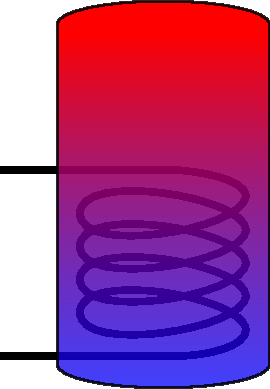
\includegraphics[width=3cm]{Thermal/images/HydraulicScheme.pdf}% of \columnwidth
%\caption{Tank with internal heat exchanger}%
%\label{tankinternal}%	
%\end{left}
%\end{figure}




\begin{equation}
mc_p \frac{dT_i}{dt}=\dot{m}_ic_p(T_{i-1} - T_i) + \dot{q}_i
\label{eq:}
\end{equation}

In this equation, $\dot{q}_i$ is composed of different heat transfer phenomena:

\begin{equation}
\dot{q}_i = \dot{q}_{conduction,~i-1} - \dot{q}_{conduction,~i} + \dot{q}_{loss,~i} +  \dot{q}_{buoyancy,~i}
\label{eq:}
\end{equation}

\begin{equation}
\dot{q}_{conduction,~i} = \frac{\lambda_{water} S}{h_{node}} (T_{i-1} - T_i) 
\label{eq:}
\end{equation}

\begin{equation}
\dot{q}_{loss,~i} = UA_{loss}(T_{i} - T_{ambient}) 
\label{eq:}
\end{equation}

\begin{equation}
\dot{q}_{buoyancy,~i} = \text{ if } (T_{i-1} \geq T_i \geq T_{i+1}) \text{ then } 0 \text{ else } ???
\label{eq:}
\end{equation}

A first attempt was to suppose that buoyancy can be modelled with an equivalent thermal conductivity. 

\begin{equation}
\text{ if } (T_{i} \leq T_{i+1}) \text{ then } \dot{q}_{buoyancy} = \lambda_{buoyancy} S (T_{i+1}-T_i)
\label{eq:}
\end{equation}

%\begin{figure}%
%\begin{left}
%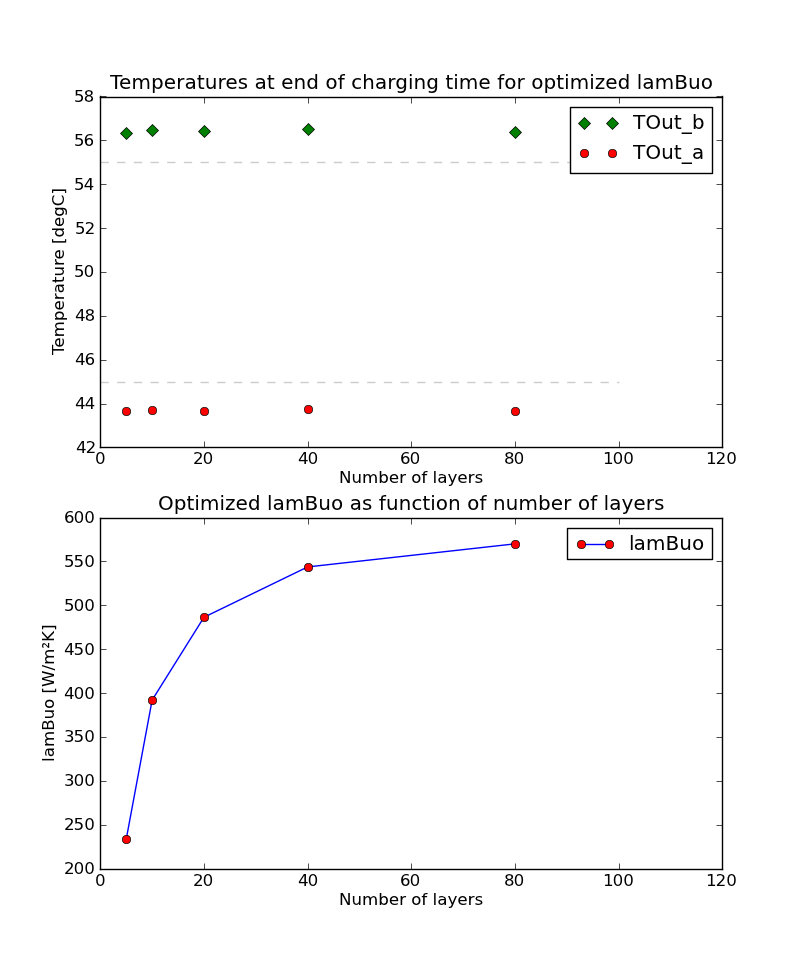
\includegraphics[width=\columnwidth]{Thermal/images/Validation_Vitocell100V390l_ChargingTimeEndTemperatures_Linear.png}% of \columnwidth
%\caption{Result of the linear parameter fitting}%
%\label{tankinternal}%	
%\end{left}
%\end{figure}

To find $\lambda_{buoyancy}$, an optimization is carried out in which for different number of nodes, the $\lambda_{buoyancy}$ that assures the best fit of the end temperatures for both charging experiments is found.

The results show that for a given number of nodes, this leads to acceptable validation results for the charging experiment.  However, the equivalent thermal conductivity is strongly dependent on the number of nodes.  As this can be due to the variable node height, mass and DT between the nodes, a model with a parameter that clearly depends on the number of nodes is not useful for sensitivity studies in which for example the tank volume and geometry is changed.

A second approach is to suppose that buoyancy is actually a mass flow rate phenomena, caused by different densities of the water as a function of temperature.  Therefore, the following equation is used as a starting point.

\begin{equation}
\text{ if } (T_{i} \leq T_{i+1}) \text{ then } \dot{q}_{buoyancy} = \dot{m}_{buo} c_p (T_{i+1}-T_i)
\label{eq:}
\end{equation}

We suppose $\dot{m}_{buo}$ depends on the temperature gradient, and is zero when the temperature difference between the layers is zero.

\begin{equation}
\dot{m}_{buo} = k_{buo} {(\frac{dT}{dh}})^{\text{exp}_{buo}}
\label{eq:}
\end{equation}

Again, optimization is used in order to identify $k_{buo}$ and $\text{exp}_{buo}$ as a function of the number of nodes. Again, we see that these coefficients are depending on the number of nodes.  We also see that the sensitivities on the obtained end temperatures in the charging experiment is large.

\begin{figure}%
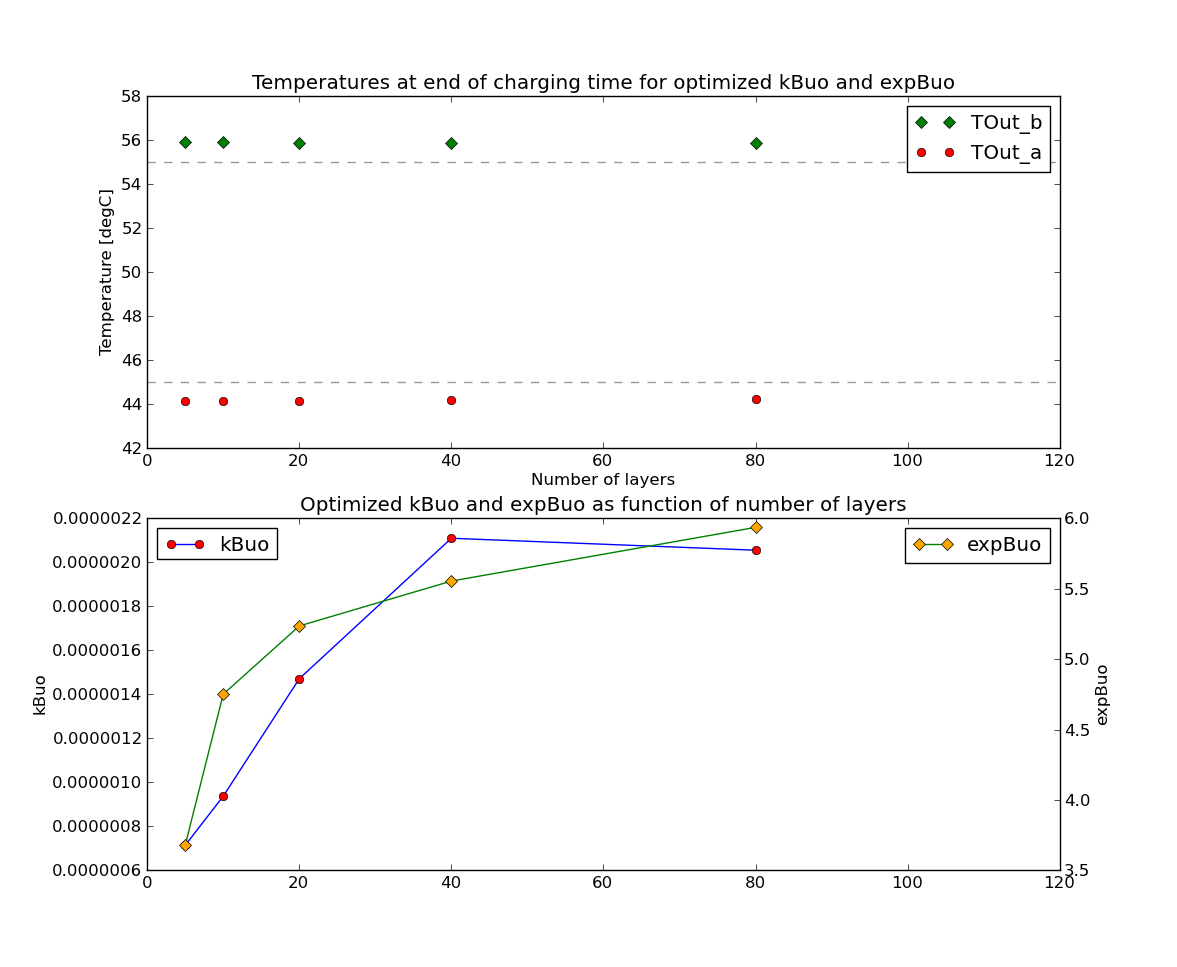
\includegraphics[width=\columnwidth]{Thermal/images/Validation_Vitocell100V390l_ChargingTimeEndTemperatures_NonLinear.png}% of \columnwidth
\caption{Result of the non-linear parameter fitting}%
\label{tankinternal}%	
\end{figure}

\begin{figure}%
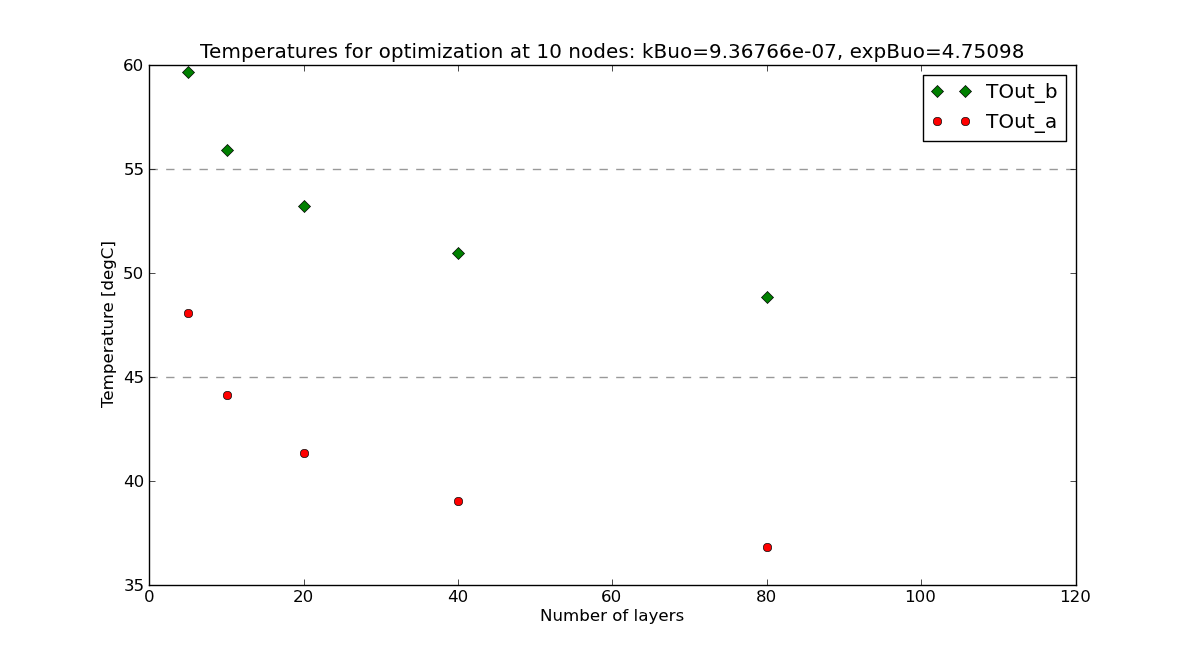
\includegraphics[width=\columnwidth]{Thermal/images/Validation_Vitocell100V390l_ChargingTimeEndTemperatures_nonlin_10nodes.png}% of \columnwidth
\caption{Resulting temperatures when the found values for 10 nodes are used}%
\label{tankinternal}%	
\end{figure}


\subsection{Heat production}

\subsubsection{Partial heater}

%\emph{IDEAS.Thermal.Components.Production.Auxiliaries.PartialDynamicHeaterWithLosses}

\vspace{6mm}

All hydraulic heater models extend from this partial heater model.  
tbc

\subsubsection{Boiler}

\subsubsection{Heat pumps}

\begin{enumerate}
	\item modulating air-source hp
	\item ground-source hp
\end{enumerate}

\subsection{Heat emission}

\subsubsection{Partial heat emission model}

%\emph{IDEAS.Thermal.Components.Emission.Auxiliaries.Partial_Emission}
\vspace{6mm}

\subsubsection{Radiator}

\subsubsection{Embedded pipe for thermally activated building systems (TABS)}

From ~\cite{Koschenz2000}

\section{Heating systems}

\subsection{Ideal heating}

\subsubsection{Hydraulic heating}

Main hydraulic scheme with replaceable models for heat production, heat emission, solar thermal system and control.

\subsection{Solar thermal system}

\subsection{Domestic hot water production}

\section{Vertical ground heat exchanger}

\subsection{Model Harm Leenders}

\subsection{Model Dieter Patteeuw}

\section{Control}


%\bibliography{Thermal/MyBibTexLibrary}












\chapter{Electricity system}
% Use \titlerunning{Short Title} for an abbreviated version of your contribution title if the original one is too long
%\author{Juan Van Roy, Bart Verbruggen and Johan Driesen}
%\authorrunning{J. Van Roy, B. Verbruggen, J. Driesen}
%\institute{Bart Verbruggen \at K.U.Leuven, Kasteelpark Arenberg 10 bus 2445, BE-3001 Leuven (Heverlee) \email{bart.verbruggen@esat.kuleuven.be}
%\and Juan Van Roy \at K.U.Leuven, Kasteelpark Arenberg 10 bus 2445, BE-3001 Leuven (Heverlee) \email{juan.vanroy@esat.kuleuven.be}}
%\maketitle

%\abstract{A numeric electric system model is developed in Modelica for integrated energy simulation.}

%\vspace{\baselineskip}

In this section, we describe in detail the electrical models that are implemented in Modelica as part of the IDEAS platform. These are models on the production, electrical distribution and storage side. First the photovoltaic (PV) system is treated which produces electricity locally from solar energy. In a second part, the distribution of electricity on distribution level is described.

Work in progress are the in-home electricity grid and the electrical storage in batteries.

\subsection{Electric power generation and distribution}

\subsubsection{Power flow analysis}

A power flow analysis is required to characterize the impact of a load profile on each connection node $n$ in the grid. A power flow analysis is performed to determine the nodal currents $\tv{i}_{n}$, the line currents $\tv{i}_{l}$ and the nodal voltages $\tv{u}_{n}$ based on the Kirchoff's circuit Laws, \ie conservation of electric charge at any node denoting that the sum of currents flowing into the node is equal to the sum of currents flowing out of the node, and conservation of energy denoting that the sum of the voltage drops around any closed circuit is zero. \\*
Denoting a complex notation for current $\tv{i} = \vert i \vert \left( \cos \tv{\theta}_{i} + \jmath \sin \tv{\theta}_{i} \right)$ st. $\tv{\theta}_{i} = \omega t + \tv{\varphi}_{i}$, for voltage $\tv{u} = \vert u \vert \left( \cos \tv{\theta}_{u} + \jmath \sin \tv{\theta}_{u} \right)$ st. $\tv{\theta}_{u} = \omega t + \tv{\varphi}_{u}$ and for impedances $Z = R + \jmath X$; the Kirchoff's circuit Laws and Ohm's Law are written as: \\*
%
\begin{gather}
\sum_{l=1}^{\mathcal{L}_{n}} \tv{i}_{n \leftarrow l} \triangleq 0 \label{kirch1} \\
\sum_{l=1}^{\mathcal{L}} \tv{u}_{\Delta_{l}} \triangleq 0 \; \mbox{st.} \; \tv{u}_{\Delta_{l}} = \tv{u}_{n_{l,1}} - \tv{u}_{n_{l,2}} = Z_{l} \tv{i}_{l}  \label{kirch2}
\end{gather}
where $\omega$ is the frequency, $\phi$ is the phase angle, $R$ is the resistance, $X$ is the reactance and wherefore line $l$ connects the nodes $n_{l,1}$ and $n_{l,2}$, and has the impedance $Z_{l}$ and wherefore $\mathcal{L}_{n}$ all lines $l$ connecting node $n$. \\*
%
When all nodal voltages and currents are known, the total flow of apparent power $\tv{S}$ at any point and the total ohmic losses can be calculated as: \\*
\begin{gather}
\tv{S} \triangleq \sum_{\phi=1}^{\mathcal{P}} \tv{P}_{\phi} + \jmath \tv{Q}_{\phi} = \sum_{\phi=1}^{\mathcal{P}} \tv{u}_{\phi} \overline{\tv{i}} : \forall \mathcal{P} = \{1\} \vee \{1,2,3,n\} \\
\tv{P}_{vi} = \sum_{l=1}^{\mathcal{L}} \sum_{\phi=1}^{\mathcal{P}} R_{\phi,l} \tv{i}_{\phi,l}^{2} : \forall \mathcal{P} = \{1\} \vee \{1,2,3,n\} \label{Ploss}
\end{gather}
where $\tv{P}$ is the active power active power, $\tv{Q}$ is the reactive power, $\tv{u}_{\phi}$ the phase voltage and $\overline{\tv{i}}$ the complex conjugate of $\tv{i}$.

\subsubsection{Transformers}

A radial distribution grid has one feeding transformer. The low-voltage (LV) side of the transformer is connected to the distribution grid, while the high-voltage (HV) side is connected to the higher-voltage grid.

A transformer (single or three-phase) is represented by the equivalent scheme as shown in Figure~\ref{figTrafo}. The transformer is represented by series ($Z_{s,HV}$ and $Z_{s,LV}$) and parallel element ($Z_{par}$). The series impedances represent the ohmic resistance and reactance (inductance) of respectively the high-voltage and low-voltage windings of the transformer. The parallel impedance represents the magnetic losses (or iron losses) in the core of the transformer. To define the active losses of the transformer, only the resistances of all impedances are taken into account.

%\begin{figure}[ht]
%\centerline{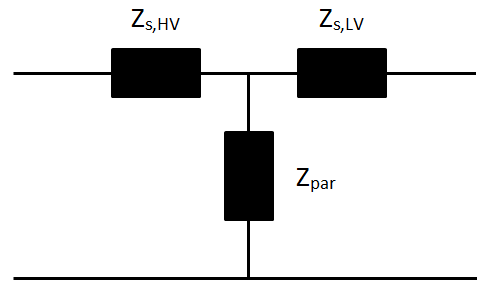
\includegraphics[width=0.65\textwidth, angle=0]{Electric/MyGraphics/trafo_equischeme.png}}
%\caption{Equivalent scheme of a transformer}
%\label{figTrafo}
%\end{figure}

The parallel element ($Z_{par}$) is defined during a no-load test of the transformer. At the primary side, the nominal voltage is applied, while the secondary windings are open. The series elements can be neglected:
\begin{equation}
Z_{par} = \left[ \frac{400}{\sqrt{3}} \right]^2 \left[ \frac{P_0}{3} \right]^{-1}
\label{3Ploss}
\end{equation}
with $P_0$ the no-load losses.

The series elements ($Z_{s,HV}$ and $Z_{s,LV}$) are defined during short-circuit tests of the transformer. During this test, the secondary windings are shorted. Since the parallel elements are large compared to the series elements, the series elements ($Z_s = Z_{s,HV} + Z_{s,LV}$)  can be defined:
\begin{equation}
Z_s = \left[ \frac{400 u_k}{100 \sqrt{3}} \right]^2 \left[ \frac{S_n u_k}{300} \right]^{-1}
\label{3Ploss}
\end{equation}
with $S_n$ the nominal apparent power of the transformer and $u_k$ the percentage of the short-circuit voltage\footnote{The short-circuit voltage is the voltage that has to be applied at the primary winding to have the nominal current in the primary winding when the secondary winding is shorted.}. Generally, $Z_s$ is evenly distributed amongst $Z_{s,HV}$ and $Z_{s,LV}$.

The active losses in a transformer are calculated as is done in Eq.~(\ref{Ploss}) for the losses in the grid. 

\subsection{Photovoltaic generation}

\subsubsection{Photovoltaic panel' power output}

The general current-voltage ($\tv{i}\tim,\tv{u}\tim$) equation for the single diode equivalent circuit is given by \\*
\begin{equation}
\tv{i}\tim = I_{ph} - I_{0} \left(\exp \frac{\tv{u}\tim + \tv{i}\tim R_{s}}{a} - 1 \right) - \frac{\tv{u}\tim + \tv{i}\tim R_{s}}{R_{sh}} \label{eq1}
\end{equation}
which can be used to determine the power output $\tv{P}\tim$ equal to $\tv{i}\tim \tv{v}\tim$ and which can be written for three points, \ie for the short-circuit, the open-circuit and the maximum power point\citep{sera}. The five required parameters are the light current $I_{ph}$, the diode reverse saturation current $I_{0}$, the series resistance $R_{s}$, the shunt resistance $R_{sh}$ and the ideality factor $a$ which depend on the cell temperature $T_{c}$, the total solar irradiation $E_{e}$ and the solar incidence angle $\xi$. \\*
%
The reverse saturation current $I_{o}$ and light current $I_{ph}$ at standard testing conditions can be found based on Eq.~(\ref{eq1}) for the short circuit (Eq.~(\ref{eq4})) and open circuit condition (Eq.~(\ref{eq5})).\\*
\begin{gather}
i_{sc} = I_{ph,\star} - I_{0,\star} \exp \frac{i_{sc} R_{s,\star}}{a_{\star}} - \frac{i_{sc} R_{s,\star}}{R_{sh,\star}} \label{eq4} \\
i_{oc} \triangleq 0 = I_{ph,\star} - I_{0,\star} \exp \frac{u_{oc}}{a_{\star}} - 
\frac{u_{oc}}{R_{sh,\star}}  \label{eq5} \\
i_{mp} = I_{ph,\star} - I_{0,\star} \left(\exp \frac{u_{mp} + i_{mp} R_{s,\star}}{a_{\star}} - 1 \right) - \frac{u_{mp} + i_{mp} R_{s,\star}}{R_{sh,\star}} \label{eq6}
\end{gather}
knowing that $(\mbox{d}ui / \mbox{d}u)\vert_{mp} = 0$ and $(\mbox{d}i / \mbox{d}u)\vert_{sc} = - R_{sh,\star}^{-1}$ \\*
%
The ideality factor has to be corrected for the cell temperature\\*
\begin{equation}
T_{c,\star} \tv{a}\tim = a_{\star} \T_{c} 
\end{equation}

The effective reverse saturation current $\tv{I}_{o}\tim$ can be derived by correcting $I_{0,\star}$ for the cell temperature $\T_{c}$ as\\*
\begin{equation}
T_{c,\star}^{3} \tv{I}_{o}\tim = I_{0,\star} \exp \left( \frac{\epsilon N}{a_{\star}}  \left(1-\frac{T_{c,\star}}{\T_{c}} \right) \right) \T_{c}^{3} 
\end{equation}

The effective light current $\tv{I}_{ph}$ can be derived by correcting $I_{ph,\star}$ for the effective irradiance $\tv{E}_{ef}^{k}$ and the cell temperature $\T_{c}$ as\\*
\begin{gather}
M_{ef,\star} E_{ef,\star} \tv{I}_{ph} = \tv{M}_{ef} \tv{E}_{ef}^{k} \left( I_{ph,\star} + \alpha_{I,sc} \left(\tv{T}_{c} - T_{c,\star}\right) \right) \\
\tv{E}_{ef}^{k} = \left( \tv{\tau}_{\xi,D} \tv{E}_{D}^{k} + \tv{\tau}_{\xi,d} \tv{E}_{d}^{k} \right) \tau_{0}^{-1} \\
\tv{\tau}_{\xi} =  \exp \frac{-f_{k} f_{l}}{\cos \tv{\xi}_{r}} \left(1 - 0.5 \frac{\sin^{2}\tv{\xi}_{r} - \tv{\xi}}{\sin^{2}\tv{\xi}_{r} + \tv{\xi}} + 0.5 \frac{\tan^{2}\tv{\xi}_{r} - \tv{\xi}}{\tan^{2}\tv{\xi}_{r} + \tv{\xi}}  \right) \label{eq7}
\end{gather}

The photovoltaic parameters are adjusted to take into account the position of the sun, the direct and indirect radiation and the ambient temperature. The cell temperature has been adjusted to be the ambient temperature plus the losses of the panel. The parameters for the non-reference conditions are calculated in the next paragraphs.\\*
%
The tilt angle and orientation of the photovoltaic panels are parameters of the PV model. Together with the sun's position, the incidence angle of the direct beam radiation can be calculated which allows to obtain the amount of radiation that gets reflected by and passes through the photovoltaic panel cover. This is done using incidence angle modifiers that are derived from De Soto et al.~\cite{desoto}. The incidence angle modifier $K_{\tau \alpha}(\xi)$ can be found from the transmittance $\tau$ of the cover system with Eq.~(\ref{eq8}), which is approximated in Eq.~(\ref{eq7}). The angle of refraction, $\theta _{r}$, is determined in Eq.~(\ref{eq6}) by Snell's law, with $\xi$ the incidence angle and $n$ the effective index of refraction of the cell cover. In Eq.~(\ref{eq7}), $f_k$ is the glazing extinction coefficient and $f_l$ is the glazing thickness. 

\subsubsection{Power output of photovoltaic system}
A photovoltaic system consists of multiple photovoltaic panels connected in series. Assuming that all photovoltaic panels are in the same condition, the output DC voltage can be multiplied by the number of photovoltaic panels in a photovoltaic system.

The number of photovoltaic panels is a parameter of the general photovoltaic system model. The peak power $P_{mp}$ is defined with $V_{mp}$, $I_{mp}$ and the number of panels $n_p$: \\*
\begin{equation}
\tv{P}_{mp} = n_p \tv{u}_{mp} \tv{i}_{mp}
\label{Ppeak}
\end{equation}

\subsubsection{Inverter}

A photovoltaic system is connected to the electrical grid through an inverter, which converts the generated DC power to AC power with an efficiency $\eta_{dc/ac}$. \\*
%
Due to the lack of simultaneity of production and consumption, a bidirectional energy flow may occur between a building and the electrical grid (\eg low voltage grid for residential buildings), which may lead to voltage instabilities on the grid (\eg increasing voltages due to the injection of electricity, unbalance, etc.). To avoid excessive feeder voltages at the moments of re-injecting photovoltaic power in the grid, the inverter is curtailed when a predefined voltage limit is reached. Curtailing of a photovoltaic system means production losses.


\section{Electrical in-home grid}
In progress.

\section{Electrical storage}
In progress.

%\begin{partbacktext}
\part{Validation or verification}
%\noindent val-i-dation (n.) 1. To declare or make legally valid. 2. To mark with an indication of official sanction. 3. To establish the soundness of; corroborate.
%\end{partbacktext}

%\title{Building energy simulation test - BESTEST}
% Use \titlerunning{Short Title} for an abbreviated version of your contribution title if the original one is too long
\author{Ruben Baetens and Dirk Saelens}
\authorrunning{R. Baetens, D. Saelens}
\institute{Ruben Baetens \at K.U.Leuven, Kasteelpark Arenberg 40 bus 2447, BE-3001 Leuven (Heverlee) \email{ruben.baetens@bwk.kuleuven.be}
\and Dirk Saelens \at K.U.Leuven, Kasteelpark Arenberg 40 bus 2447, BE-3001 Leuven (Heverlee) \email{dirk.saelens@bwk.kuleuven.be}}
\maketitle

\section{Introduction}

The thermal building model are \emph{validated} by comparative tests based on the \emph{Building Energy Simulation Test} (BESTEST)~\cite{Judkoff1995, Neymark2008} as developed under supervision of the International Energy Agency (IEA)~\cite{Lomas1994,Lomas1994a} and standardized as the ANSI/ASHRAE Standard 140-2007~\cite{ASHRAE140}. This standard consists of a series of specified test cases and has been developed to diagnose whole building energy simulation software. Here, output values such as the annual energy consumptions, peak loads, average and extreme room air temperatures, and some hourly data are compared to miscellaneous building energy simulation programs, e.g. BLAST, DOE2.1D, ESP-R, SERIRES / SUNCODE, S3PAS, TASE and TRNSYS. 

\subsection{Building energy simulation test cases}

Within this work, the so-called \emph{“basic test cases} are used” to \emph{validate} the building model. These test cases test the ability to model combined effects as thermal mass, solar gains and solar shading, air infiltration, internal heat gains, sunspaces and thermostat control. Three series of basic cases are tested :

\begin{enumerate}
\item Qualification cases 600 to 650 representing a set of lightweight buildings that are relatively realistic with respect to their thermal characteristics. Within this set of cases, case 600 tests the south solar transmission, case 620 tests the east and west solar transmittance and incidence, case 640 tests night setback and case 650 tests venting.
\item Qualification cases 900 to 960 representing a set of heavyweight buildings that are relatively realistic with respect to their thermal caracteristics and include a building configuration with a sunspace. Within this set of cases, case 900 tests the thermal mass and solar interaction, test 920 tests the east and west transmittance and its mass interaction, case 940 tests night set-back and its mass interaction, case 950 tests venting and its mass interaction and case 960 tests passive solar and interzonal heat transfer.
\item Free-float basic test cases 600FF, 900FF, 650FF and 950FF equaling the corresponding non-FF cases except the absence of a mechanical heating or cooling systems.
\end{enumerate}

%Add all tests on ground slabs too

\subsection{Test results}

\subsubsection{Annual heating and cooling loads}

\begin{figure}[ht]
\subfigure[Annual heating loads for the low mass and heavy mass buildings.]{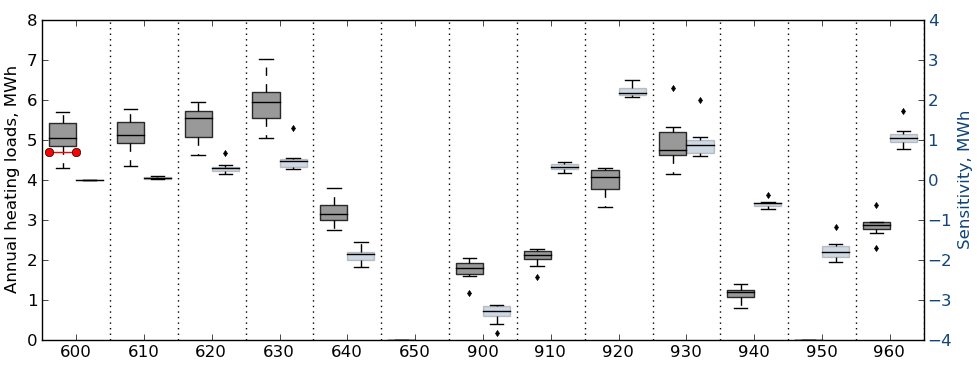
\includegraphics[width=\textwidth]{Buildings/MyGraphics/AH_BESTEST.png}\label{fig:AH_BESTEST}}
\subfigure[Annual sensible cooling loads for the low mass and heavy mass buildings.]{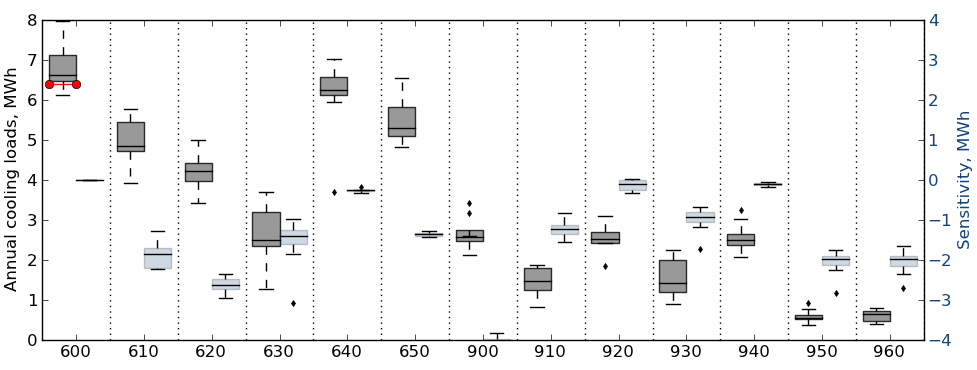
\includegraphics[width=\textwidth]{Buildings/MyGraphics/AC_BESTEST.png}\label{fig:AC_BESTEST}}
\caption{Annual heating and sensible cooling loads for the low mass and heavy mass buildings.} 
\end{figure}

\subsubsection{Peak heating and cooling loads}

\begin{figure}[t]
 \center
 \begin{tikzpicture}
\begin{axis} [
 width=12.8cm, height=4.9cm,
 xmin=-0.8, xmax=13.8,
 ymin=-0.1,  ymax=1.6,
 scatter/classes={a={darkgray,scale=0.7,opacity=0.4},b={darkgray,mark=o,scale=0.7,opacity=0.4}}, 
 xtick={0,1,2,3,4,5,6,7,8,9,10,11,12,13},
 xticklabels={\eg,600,610,620,630,640,650,900,910,920,930,940,950,195},]
 \addplot[scatter, only marks, scatter src=explicit symbolic] table [x=x,y=y1,meta=label]{./data/bestest.dat};
 \addplot[scatter, only marks, scatter src=explicit symbolic] table [x=x,y=y2,meta=label]{./data/bestest.dat};
 \addplot[scatter, only marks, scatter src=explicit symbolic] table [x=x,y=y3,meta=label]{./data/bestest.dat};
 \addplot[scatter, only marks, scatter src=explicit symbolic] table [x=x,y=y4,meta=label]{./data/bestest.dat};
 \addplot[scatter, only marks, scatter src=explicit symbolic] table [x=x,y=y5,meta=label]{./data/bestest.dat};
 \addplot[scatter, only marks, scatter src=explicit symbolic] table [x=x,y=y6,meta=label]{./data/bestest.dat};
 \addplot[scatter, only marks, scatter src=explicit symbolic] table [x=x,y=y7,meta=label]{./data/bestest.dat};
% \addplot coordinates {(-1, 0.9)(15, 0.9)};
 \addplot coordinates {(-1, 1)(15, 1)};
 %reference
 \addplot[color=black,mark=halfcircle*] coordinates {(-0.24, 1.05)(-0.08, 1.1)(0.08, 0.95)(0.24, 0.9)};
 \node[pin=90:{\footnotesize $Q_{h}$}] at (axis cs:-0.24,1.05) {};
 \node[pin=90:{\footnotesize $P_{h}$}] at (axis cs:0.08,0.95) {};
 \node[pin=-90:{\footnotesize $Q_{c}$}] at (axis cs:-0.08,1.1) {};
 \node[pin=-90:{\footnotesize $P_{c}$}] at (axis cs:0.24,0.9) {};
 \node[pin=180:{\footnotesize \textsc{bestest}}] at (axis cs:3.92,1.403) {};
 %case600
 \addplot[color=black,mark=halfcircle*] coordinates {(0.76, 1.038)(0.92, 0.972)(1.08, 0.967)(1.24, 1.029)}; %wettercorr
 %case610
 \addplot[color=black,mark=halfcircle*] coordinates {(1.76, 1.034)(1.92, 0.944)(2.08, 0.967)(2.24, 0.961)}; %wettercorr
 %case620
 \addplot[color=black,mark=halfcircle*] coordinates {(2.76, 0.987)(2.92, 0.906)(3.08, 0.952)(3.24, 0.974)}; %wettercorr
 %case630
 \addplot[color=black,mark=halfcircle*] coordinates {(3.76, 0.943)(3.92, 1.045)(4.08, 0.966)(4.24, 0.998)}; %wettercorr
 %case640
 \addplot[color=black,mark=halfcircle*] coordinates {(4.76, 1.000)(4.92, 1.078)(5.08, 1.091)(5.24, 1.036)}; %wettercorr
 %case 650
 \addplot[color=black,mark=halfcircle*] coordinates {(5.92, 1.094)(6.24, 1.048)}; %wettercorr
 %case900
 \addplot[color=black,mark=halfcircle*] coordinates {(6.76, 0.828)(6.92, 0.797)(7.08, 0.906)(7.24, 0.828)}; %wettercorr
 %case910
 \addplot[color=black,mark=halfcircle*] coordinates {(7.76, 0.792)(7.92, 0.636)(8.08, 0.862)(8.24, 0.808)}; %wettercorr
 %case920
 \addplot[color=black,mark=halfcircle*] coordinates {(8.76, 0.839)(8.92, 0.787)(9.08, 0.874)(9.24, 0.846)}; %wettercorr
 %case930
 \addplot[color=black,mark=halfcircle*] coordinates {(9.76, 0.781)(9.92, 0.906)(10.08, 0.878)(10.24, 0.884)}; %wettercorr
 %case940
 \addplot[color=black,mark=halfcircle*] coordinates {(10.76, 0.718)(10.92, 0.787)(11.08, 0.820)(11.24, 0.868)}; %wettercorr
 %case950
 \addplot[color=black,mark=halfcircle*] coordinates {(11.92, 1.023)(12.24, 0.956)}; %wettercorr
 %case195
 \addplot[color=black,mark=halfcircle*] coordinates {(12.76, 0.98)(12.92, 1.1096)(13.08, 0.9893)(13.24, 1.0692)}; %wettercorr
\end{axis}
\end{tikzpicture}
 \caption{Verification by \abb{bestest}' inter model comparison, denoting the annual heating loads $Q_{h}$, the annual cooling loads $Q_{c}$, the hourly integrated peak heating loads $P_{h}$ and hourly integrated peak cooling loads $P_{c}$ normalized by the all-code mean for the low and heavy mass base cases.}
\end{figure}

%\begin{figure}[ht]
%\subfigure[Peak heating loads for the low mass and heavy mass buildings.]{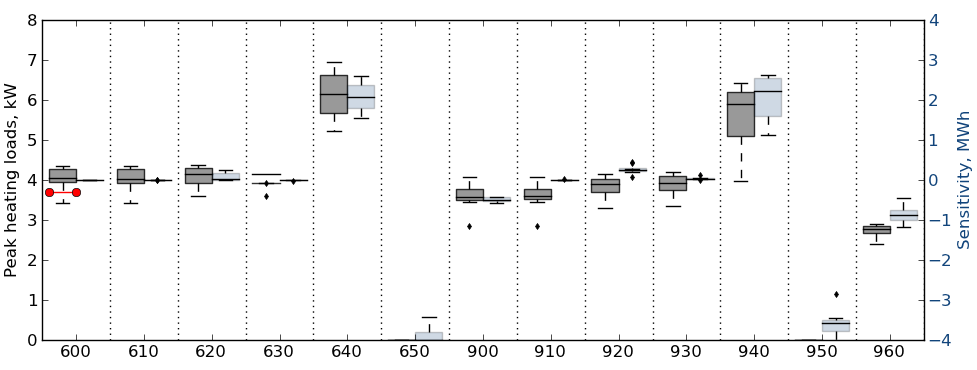
\includegraphics[width=\textwidth]{Buildings/MyGraphics/PH_BESTEST.png}\label{fig:PH_BESTEST}}
%\subfigure[Peak sensible cooling loads for the low mass and heavy mass buildings.]{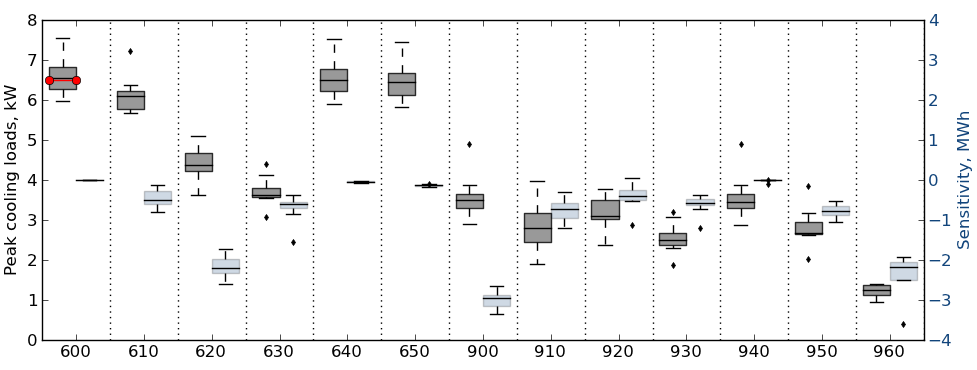
\includegraphics[width=\textwidth]{Buildings/MyGraphics/PC_BESTEST.png}\label{fig:PC_BESTEST}}
%\caption{Peak heating and sensible cooling loads for the low mass and heavy mass buildings.} 
%\end{figure}

\subsubsection{Indoor air temperatures}

\begin{figure}[ht]
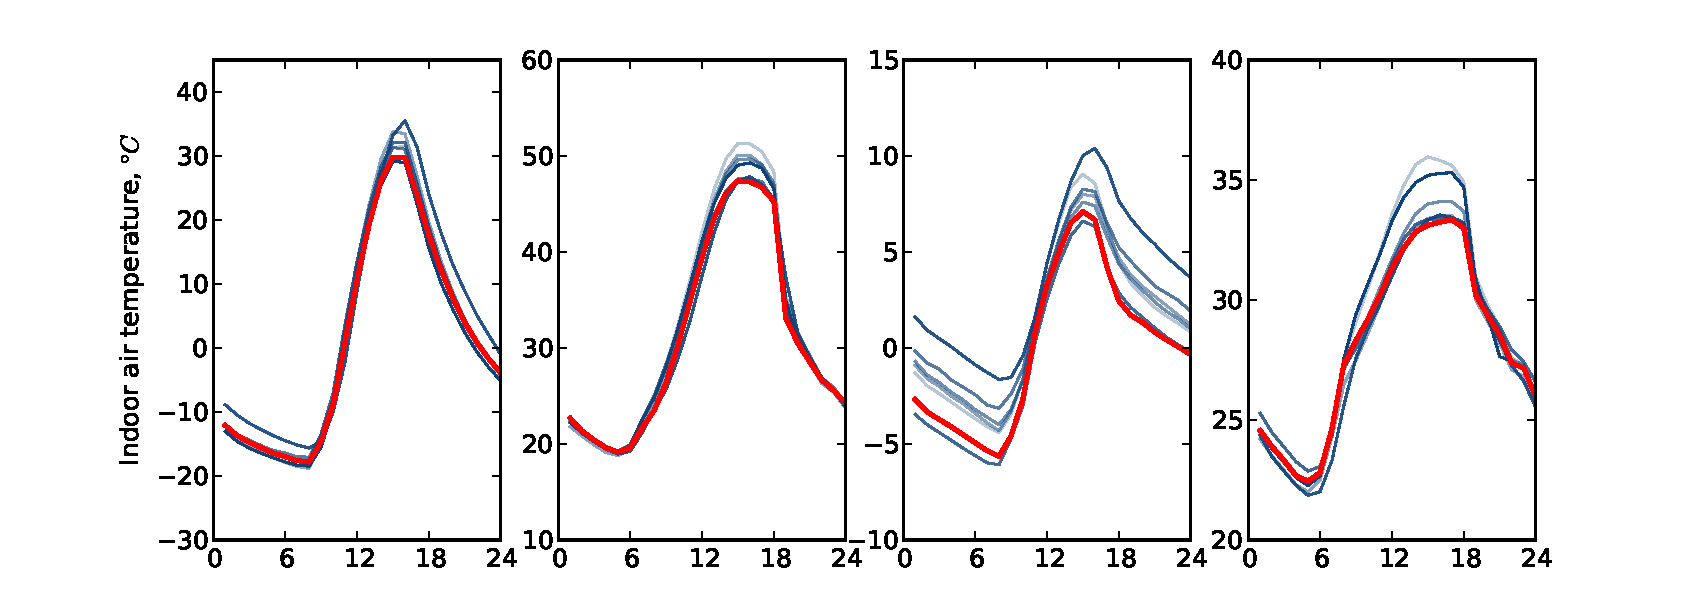
\includegraphics[width=\textwidth]{Buildings/MyGraphics/Temp_BESTEST.pdf}
\label{fig:Temp_BESTEST}
\caption{Indoor temperatures for the low mass and heavy mass buildings.} 
\end{figure}

%\bibliography{Buildings/MyBibTexLibrary}




%
\title{Thermal building energy system test - BESTEST}
% Use \titlerunning{Short Title} for an abbreviated version of your contribution title if the original one is too long
\author{Roel De Coninck and Lieve Helsen}
\authorrunning{R. De Coninck, L. Helsen}

\maketitle

\abstract{A numeric thermal system model is developed in Modelica for integrated energy simulation.}

%\bibliography{Thermal/MyBibTexLibrary}











%
\title{IEEE Distribution system analysis for radial test feeders }
% Use \titlerunning{Short Title} for an abbreviated version of your contribution title if the original one is too long
\author{Juan Van Roy, Bart Verbruggen and Johan Driesen}
\authorrunning{J. Van Roy, B. Verbruggen, J. Driesen}

\maketitle

\abstract{A numeric electric system model is developed in Modelica for integrated energy simulation.}

%\bibliography{Electric/MyBibTexLibrary}











%\begin{partbacktext}
\part{Bibliography}
%\noindent bib·li·og·ra·phy (n.) 1. A list of the works of a specific author or publisher. 2. a. A list of writings relating to a given subject: a bibliography of Latin American history. b. A list of writings used or considered by an author in preparing a particular work. 3. a. The description and identification of the editions, dates of issue, authorship, and typography of books or other written material. b. A compilation of such information.
%\end{partbacktext}

%\bibliography{Climate/MyBibTexLibrary,Buildings/MyBibTexLibrary,Electric/MyBibTexLibrary,Thermal/MyBibTexLibrary} 

{\footnotesize
\bibliography{Climate/MyBibTexLibrary,Buildings/MyBibTexLibrary,Electric/MyBibTexLibrary,Thermal/MyBibTexLibrary}{}
\bibliographystyle{ieeetr}}

\backmatter%%%%%%%%%%%%%%%%%%%%%%%%%%%%%%%%%%%%%%%%%%%%%%%%%%%%%%%
%\appendix
%\include{appendix}

%\printindex

%%%%%%%%%%%%%%%%%%%%%%%%%%%%%%%%%%%%%%%%%%%%%%%%%%%%%%%%%%%%%%%%%%%%%%



\end{document}





